\documentclass[a4paper, 11pt]{book}
\usepackage{/home/nora/Documents/Enseignement/Prepa/bpep/fichiers_utiles/preambule}

\makeatletter
\renewcommand{\@chapapp}{Kh\^olles MPSI -- semaine}
\makeatother
\renewcommand\thechapter{17}

% \toggletrue{corrige}  % décommenter pour passer en mode corrigé

% IMPORTS automatiques
\newcommand{\f}[2]{{
		\mathchoice
		{\dfrac{#1}{#2}}
		{\dfrac{#1}{#2}}
		{\frac{#1}{#2}}
		{\frac{#1}{#2}}
}}

\newcommand{\e}[1]{{}_{\text{#1}}}

\usepackage{physics}

 % fin des IMPORTS automatiques

\begin{document}

\chapter{Sujet 1\siCorrige{\!\!-- corrig\'e}}

\subimport{/home/nora/Documents/Enseignement/Prepa/bpep/exercices/Colle/ressort_poids/}{sujet.tex}

\chapter{Sujet 2\siCorrige{\!\!-- corrig\'e}}

Énoncer et démontrer les théorèmes de la puissance mécanique et de l'énergie
mécanique.

\resetQ
\section{Positions d'équilibre d'un anneau sur un cercle}
\enonce{%
  \noindent
	\begin{minipage}{0.60\linewidth}
		Un anneau assimilable à un point matériel M de masse $m$ peut glisser sans
		frottement sur une glissière circulaire de rayon $R$ et de centre O.
		L'anneau est attaché à un ressort de raideur $k$ dont une extrémité est
		fixée à la glissière au point A. Sa position est repérée par l'angle $\tt$
		entre le rayon OM et l'axe horizontal (O$x$). Pour simplifier les calculs,
		on considérera que la longueur à vide $\ell_0$ du ressort est nulle.
	\end{minipage}
	\hfill
	\begin{minipage}{0.35\linewidth}
		\begin{center}
			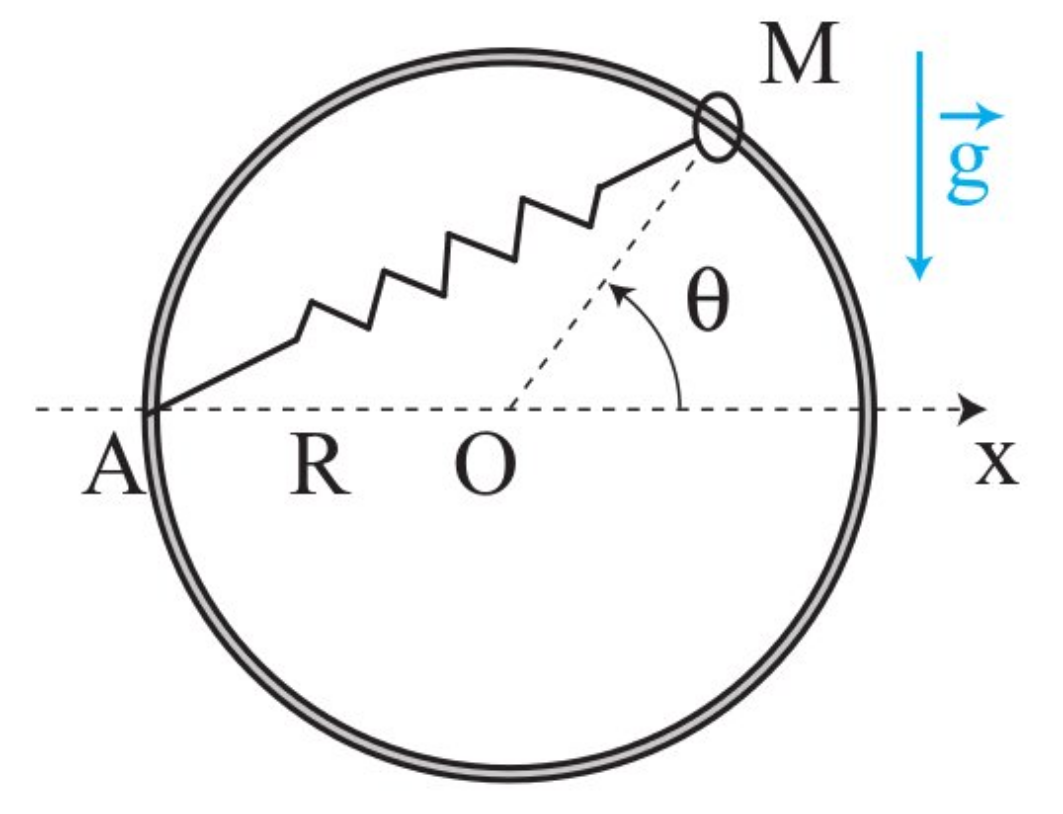
\includegraphics[width=.9\linewidth]{../figures/anneau_cercle_ressort-plain}
		\end{center}
	\end{minipage}
}

\QR{%
	Montrer que la longueur $\ell$ s'exprime $\ell = R\sqrt{2(1+\cos\tt)}$.
}{%
	\begin{minipage}[t]{0.25\linewidth}
		~
		\begin{center}
			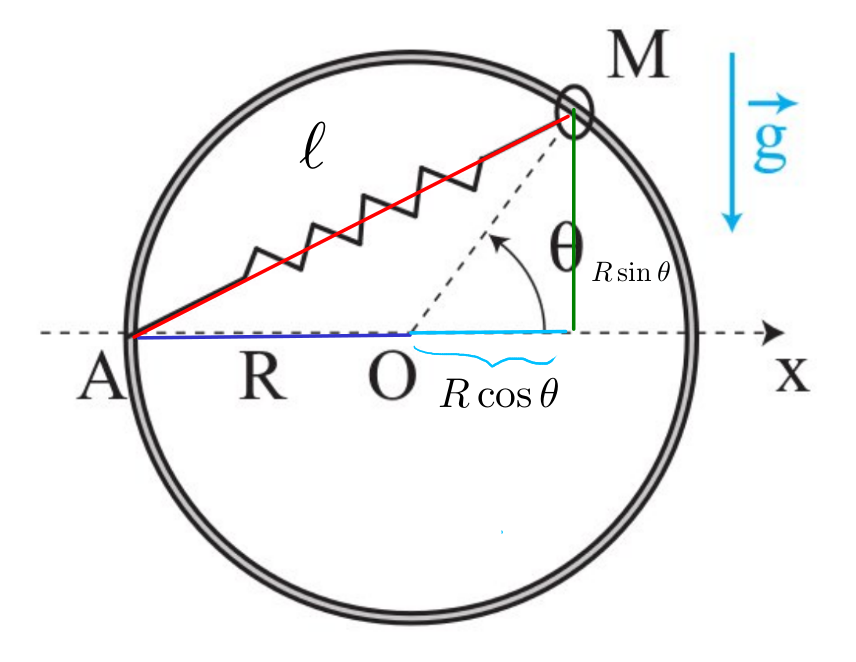
\includegraphics[width=\linewidth]{../figures/anneau_cercle_ressort-proj}
			\captionsetup{justification=centering}
			\captionof{figure}{Détermination de $\ell$}
			\label{fig:anncercproj}
		\end{center}
	\end{minipage}
	\hfill
	\begin{minipage}[t]{0.70\linewidth}
		On peut réutiliser la relation de \textsc{Chasles} pour écrire
		$\vv{\rm AM} = \vv{\rm AO} + \OM$ et déterminer la distance en prenant
		la norme, mais ici une simple utilisation du théorème de
		\textsc{Pythagore} suffit. On projette M sur l'axe $x$ pour avoir
		\begin{align*}
			\ell^2       & = (R+R\cos\tt)^2 + (R\sin\tt)^2
			\\\Lra
			\ell^2       & = R^2 + 2R^2\cos\tt + R^2(\cos^2\tt + \sin^2\tt)
			\\\Lra
			\ell^2       & = 2R^2(1+\cos\tt)
			\\\Lra
			\Aboxed{\ell & = R\sqrt{2(1+\cos\tt)}}
			\qed
		\end{align*}
	\end{minipage} \bigbreak
}
\QR{%
	Exprimer l'énergie potentielle $\Ec_p$ du système constitué de
	l'anneau et du ressort en fonction de l'angle $\tt$.
}{%
	L'énergie potentielle totale $\Ec_p$ est constituée de l'énergie
	potentielle de pesanteur de l'anneau et de l'énergie potentielle
	élastique du ressort. Pour $\Ec_{p,p}$ avec origine en O, on a une
	altitude $R\sin\tt$~; pour $\Ec_{p,el}$ on a la différence de longueur à
	a vide $\ell -\ell_0$ avec $\ell_0 = 0$, d'où
	\begin{align*}
		\Ec_p         & = \Ec_{p,p} + \Ec_{p,el}
		\\\Lra
		\Ec_p         & = mgR\sin\tt + \frac{k}{2}\ell^2
		\\\Lra
		\Aboxed{\Ec_p & = mgR\sin\tt + kR^2(1+\cos\tt)}
		\qed
	\end{align*}
}
\QR{%
	Déterminer les positions d'équilibre de l'anneau.
}{%
	On trouve les positions d'équilibre de l'anneau en trouvant les angles
	$\tt\ind{eq}$ tels que la dérivée de $\Ec_p$ s'annule, soit
	\begin{align*}
		\eval{\dv{\Ec_p}{\tt}}_{\tt\ind{eq}} & = -kR^2\sin\tt\ind{eq} +
		mgR\cos\tt\ind{eq} = 0
		\\\Lra
		\sin\tt\ind{eq}                      & = \frac{mg\cancel{R}}{kR^{\cancel{2}}}\cos\tt\ind{eq}
		\\\Lra
		\tan\tt\ind{eq}                      & = \frac{mg}{kR}
		\\\Lra
		\boxed{\tt_{\equ,1} = \arctan(\frac{mg}{kR})}
		\quad                              & \text{et}\quad
		\boxed{\tt_{\equ,2} = \pi + \arctan(\frac{mg}{kR})}
		\qed
	\end{align*}
	avec $\tt_{\equ,1}$ compris entre 0 et \ang{90}, et $\tt_{\equ,2}$ compris
	entre 180 et \ang{270}.
}
\QR{%
	Préciser si les positions d'équilibre obtenues sont stables.
}{%
	On étudie la stabilité des positions en évaluant la dérivée seconde de
	$\Ec_p$ en ce point et en vérifiant son signe. On obtient
	\begin{align*}
		\eval{\dv[2]{\Ec_p}{\tt}}_{\tt\ind{eq}} & = -kR^2\cos\tt\ind{eq}
		-mgR\sin\tt\ind{eq}
		\\\Lra
		\eval{\dv[2]{\Ec_p}{\tt}}_{\tt\ind{eq}} & = -\left(kR^2 +
		\frac{m^2g^2}{k}\right)\cos\tt\ind{eq}
	\end{align*}
	en utilisant les résultats précédents sur la dérivée première de
	$\Ec_p$. L'intérieur de la parenthèse étant positif, le signe de cette
	dérivée seconde est opposé à celui du cosinus de la position
	d'équilibre. Or,
	$\cos\tt_{\equ,1} > 0$ et $\cos\tt_{\equ,2} < 0$, donc
	\begin{gather*}
		\boxed{\eval{\dv[2]{\Ec_p}{\tt}}_{\tt_{\equ,1}} < 0}
		\qet
		\boxed{\eval{\dv[2]{\Ec_p}{\tt}}_{\tt_{\equ,2}} > 0}
		\qed
	\end{gather*}
	La première position est donc instable, et la seconde stable.
\begin{center}
	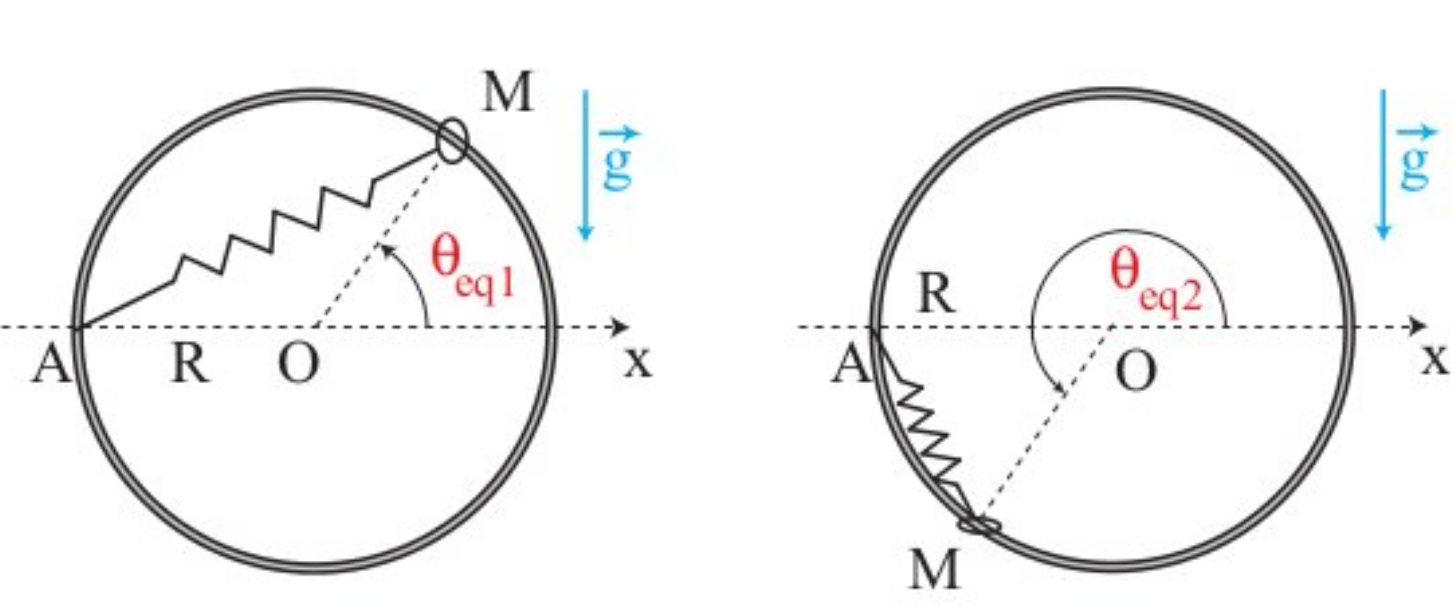
\includegraphics[width=.5\linewidth]{../figures/anneau_cercle_ressort-corr_eq}
  \captionof{figure}{Positions d'équilibre du système}
	\label{fig:anncerccorr}
\end{center}
}

\chapter{Sujet 3\siCorrige{\!\!-- corrig\'e}}

\resetQ
\subimport{/home/nora/Documents/Enseignement/Prepa/bpep/exercices/TD/frottement_quadratique/}{sujet.tex}

\chapter{Sujet 4\siCorrige{\!\!-- corrig\'e}}
\resetQ
\subimport{/home/nora/Documents/Enseignement/Prepa/bpep/exercices/TD/marsupilami/}{sujet.tex}

\end{document}
